\chapter{Megvalósítás}

\section{Előkészület}

Mivelhogy Androidos alkalmazásom kezdeti része nagy mértkében hagyatkozik a Firebase által nyújtott szolgáltatásokra, fontos ezeket megvalósítani a program létrehozásának megkezdése előtt.
\begin{itemize}
    \item Először is szükségünk lesz egy Firebase regisztrációra.
    \item Sikeres regisztráció után létre kell hoznunk egy Firebase projektet, ami az alkalmazásunk felhő alapú szolgáltatásait hivatott megvalósítani.
\end{itemize}

Ezen a ponton érdemes létrehozni az Android Studio projectet, ugyanis a Firebase-nak szüksége van a project adataira a sikeren háttérszolgáltatások ellátásához.

Szükségünk lesz az Android Studio programra, ahol a munka nagy része zajlani fog.
Ezt a hivatalos weboldalról\cite{AndroidStudio} tudjuk ingyenesen beszerezni.
Ezután a programot fel kell telepíteni, majd használatba is vehetjük.
Miután beléptünk a programba, az első dolgunk egy új project létrehozása, amit a GUI-n keresztül a bal felső sarokban lévő \textbf{File>New project} útvonalon találunk meg.
Továbbiakban a projekt létrehozási képernyőre\ref{fig:newproject} leszünk irányítva, ahol kiválaszthatjuk programunk alapvető felépítését, avagy a vázát.

\begin{figure}[h]
\centering
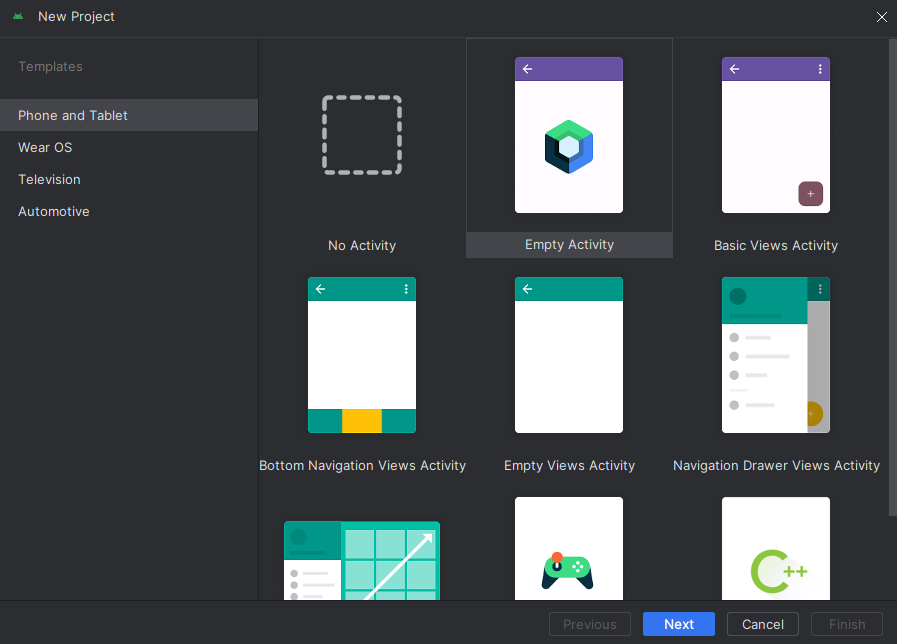
\includegraphics[scale=0.4]{images/android studio.png}
\caption{Projekt létrehozási ablak.}
\label{fig:newproject}
\end{figure}

Itt az IDE több lehetőséget is felkinál, én az \texttt{Empty Activity} sémát használom. Ebben a módban az Android Studio elkészíti nekünk az alap felépítését, függőségeit a programnak, ezáltal nekünk nem kell bajlódni a beállításokkal.
Ha ez megvan, akkor sikeresen létrehoztuk a projektünket az Android Studio keretein belül, ami biztosítja nekünk a futtathatóságot.

Miután létrehoztuk az Android Studio Projektet vissza kell mennünk a Firebase-en létrehozott projektünk oldalára, és hozzá kell rendelnünk a számítógépünkön létrehozott projekthez.
Ezt egész egyszerűen megtehetjük, a hozzáadásnál csak a gyökérkönyvtár nevét (esetünkben
\texttt{eu.thesis.onlinecatchlog}) kell megadni, ezzel elkezdtük a háttérszolgáltatás kiépítését.
Következő lépésként az Authentication fület lenyitva hozzá kell adnunk a projektünkhöz, majd bekapcsolni az E-mail, és jelszó alapú bejelentkeztetést. Ezután már csak annyi van hátra a Firebase Console-on belül, hogy létrehozunk egy teszt fiókot, amivel az alkalmazás fejlesztése közben tesztelni tudjuk majd a funkciók működését.
Ezután érdemes letölteni a Firebase által kínált \texttt{google-services.json} nevezetű fájlt, amit el kell helyeznünk a projekt mappába. Ezáltal a későbbiekben hozzáadott funkciók össze tudnak kapcsolódni a felhőben létrehozott adatokkal.

Ennek az elvégzése után térjünk vissza az Android Studio felületére, ugyanis a projektünkben még nem inicializáltuk a Firebase-t. Ezt érdemes még a fejlesztési szakasz elején megtenni, ugyanis a külső könyvtár segítségével fogunk hivatkozni például a bejelentkezési képernyőn bevitt adatokra.

\begin{figure}[h]
\centering
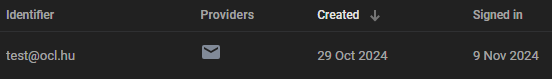
\includegraphics[scale=1]{images/firebaseloginadd.png}
\caption{A létrehozott tesztfiók.}
\label{fig:firebaseloginadd}
\end{figure}

A Firebase Console-ban további érdekes funkciókat is láthatunk, például használatra vonatkozó statisztikákat mutat ki, naplózza az alkalmazásunkhoz tartozó használati adatokat, amik nagyon fontosak a publikálás után. Így teljesebb képet kaphatunk a valós alkalmazás használati adatokról.

Mindezek után nyissunk egy terminált a projekt mappájában. Erre lehetőséget kínál közvetlen az Adnroid Studio is, így azt érdemes használni.

Projektünk még nem áll közvetlen összeköttetésben a szerverrel, ezért most inicializálni kell a Firebase-t a projekten belül.

A terminálba írjuk be a következőt:

\begin{verbatim}
    npm install -g firebase-tools
\end{verbatim}

Ezzel feltelepítjük a szükséges fájlokat a lokális szerver üzemeltetéséhez, amin belül tesztelni fogjuk az alkalmazásunkat.

Következőnok fontos, hogy az alkalmazás gyökérmappájába legyünk, használjuk az alábbi parancsot:
\begin{verbatim}
    firebase init
\end{verbatim}

Ezzel létrehoztunk a Firebase-nek szükséges fájlokat a projektünkben.
\begin{verbatim}
    firebase login
\end{verbatim}
Majd be kell jelentkeznünk a weboldalon megadott információkkal, hogy hitelesítsük magunkat.
\section{Android Studio projektek felépítése}

\subsection{Könyvtárak}

\textbf{Java/Kotlin könyvtár:} 
Itt található minden olyan fájl amely az alkalmazás fő logikáját hivatott megvalósítani.
Ezt hívjuk forráskódnak. A három fő csomag sorrendben \texttt{com.example.yourappname}. Ez a gyökércsomag, ami tartalmaz minden olyan Kotlin fájlt, amely elengedhetetlen alkalmazásunk futtatásához. Többet között itt található meg a korábban említett \textbf{MVVM} fájlok is.
Fontos kiemelni, hogy a régebbi architektúrát alkalmazó, legacy kódok másmilyen elrendezésűek.

\textbf{res könyvtár:}
Az alkalmazáshoz szükséges forrásokat itt találjuk, amik az olvashatóságot hivatottak megkönnyíteni, illetve a kódismétlést szeretnék minimalizálni. Minden olyan UI elemen megjelenített \textbf{String} vagy \textbf{kép}, vagy \textbf{ikon}-t itt kell deklarálni.
Ennek a könyvtárnak az előbbiek alapján három fő egysége van: 
\begin{itemize}
    \item \texttt{drawable}, ahol megadhatjuk a az alkalmazásunkban használatos képeket, vektorgrafikus elemeket.
    \item \texttt{values}, ahol deklarálhatjuk a különböző sűrűn előforduló stringeket, színeket, és stílusokat.
    \item \texttt{mipmap}, ahol pedig az alkalmazás ikonjait tudjuk beállítani.
\end{itemize}
Az itt megtalálható deklarációkra a fejlesztés következő szakaszaiban csak hivatkozni kell.
Ezekhez a forrás fájlokhoz mi is hozzáadhatunk változókat, sőt fontos is hogy minimalizáljuk a kód ismétlést.

\subsection{Gradle}

Itt kettő fő komponenst kell megkülönböztetni: a \texttt{projekt} szintű, és az \texttt{app} szintű gradle fájlokat. Az előbbi fájl tartalmazza a projektünk moduljainak beállítasait, itt állíthatjuk be a különböző Gradle és Android Plugin verziókat. Az utóbbi az érdekesebb számunkra, ugyanis itt állíthatjuk be a specifikus függőségeket, megadhatjuk a minimum Android verziót, illetve SDK verziót, nem utolsó sorban különböző külső könyvtárakat importálhatunk, amivel szélesíthetjük alkalmazásunk funkcionalitását, és megkönnyíthetjük a fejlesztés folyamatát.

\subsection{Manifest}

Ennek a fájlnak régebben sokkal nagyobb jelentősége volt, ugyanis minden egyes oldalt amit létrehoztunk innen tudtunk inicializálni, alapvető funkciókat beállítani. Az új MVVM architektúra használatával ennek a fájlnak lényegében annyi szerepe maradt számunkra, hogy innen indítjuk el az alkalmazásunkat megnyitáskor.
\newpage

\begin{java}[caption = {AndroidManifest.xml fájl egy részlete}]
<activity
    android:name=".MainActivity"
    android:exported="true"
    android:label="@string/app_name"
    android:theme="@style/Theme.ThesisExamples">
    <intent-filter>
  <action android:name="android.intent.action.MAIN"/>

  <category android:name="android.intent.category.LAUNCHER"/>
    </intent-filter>
</activity>
\end{java}

Ahogy az alábbi programkód részleten láthatjuk, a \texttt{MainActivity.kt} nevű fájlt inicializálni kell az \texttt{AndroidManifest.xml} nevezetű fájlban, ugyanis az alkalmazás indításakor itt kerül inicializálásra az első képernyő, ami jelen esetünkben a \texttt{MainActivity}. Ezt a beállítást az \texttt{<intent-filter>} változóval tudjuk megtenni, ahol a \texttt{<category android:name="android.intent.category.LAUNCHER"/>} beállítással megmondjuk a programnak, hogy ez a kezdőpont.

\section{Az alkalmazás létrehozása}

A projekt létrehozása után egy üres keretet kaptunk, ami futtatható, azonban sok minden nincs rajta. Miután az előkészületekben megteremtettünk minden előleges feltételt, hogy alkalmazásunkat el kezdjük fejleszteni, nincs más hátra mint a programozás.

\subsection{MainActivity.kt}

\begin{java}[caption = {MainActivity.kt fájl egy részlete}]
@AndroidEntryPoint
class MainActivity : ComponentActivity() {
    override fun onCreate(savedInstanceState: Bundle?) {
        super.onCreate(savedInstanceState)
        configureFirebaseServices()

        setContent { MainApp() }
    }

    private fun configureFirebaseServices() {
        if (BuildConfig.DEBUG) {
            Firebase.auth.useEmulator(LOCALHOST, AUTH_PORT)
            Firebase.firestore.useEmulator(
            LOCALHOST, FIRESTORE_PORT)
        }
    }
}
\end{java}

Ennél a fájlnál részletesebben kiszeretnék térni a szerkezetre, illetve a leírt kódra, mivel ez adja egy nagyon kritikus részét az alkalmazásunknak. Miután az \newline
\texttt{AndroidManifest.xml}-nél beállította az IDE ezt a kezdőpontot, itt kell inicializálnunk az alkalmazást, és a Firebase-t.
\begin{itemize}
    \item Az \textbf{@AndroidEntryPoint} annotiáció jelzi a Hilt számára, hogy ez az activity egy belépési pont, azaz injektálni kell a függőségeket, amik később kellenek az alkalmazás számára.
    \item A \textbf{MainActivity} osztály a \textbf{ComponentActivity}-t örökli, amely az Androidos fejlesztői környezet egy alapl Activity-je. Szerepe különösen fontos a későbbi \textbf{@Compose} annotációkban, ugyanis ez lesz felelős a képernyő frissítésének.
    \item \textbf{onCreate} metódus: ez az Activity életciklusának kezdő pontja. Itt inicializálódik az alkalmazás. Ebben a részben hívjuk meg a 
    \textbf{configureFirebaseServices()} függvényt, amely konfigurálja a lokális tesztelést.
    \item A \textbf{setContent} meghívásával beállítjuk a felhasználói felületet, aminek a motorja a \textbf{MainApp()}.
\end{itemize}

\subsection{MainApp.kt}

A \textbf{MainApp()} függvény az alkalmazás központi függvénye, fő komponense. Ebben a függvényben állítjuk be a témát amit előre meghatároztunk, illetve a navigációs keretet is itt inicializáljuk.
A témát (\textbf{OnlineCatchLogTheme}) amit ebben a blokkban kiválasztunk az összes navigációs komponensre alkalmazni fogjuk. Ez magában foglalja a színeket, és betűtípusokat, és az éjszakai módot is.

\begin{java}[caption = {MainApp.kt fő függvény leírása.}]
@Composable
fun MainApp() {
    OnlineCatchLogTheme{
    
    }
}
\end{java}

A NavHost függvénnyel meghívjuk a \textbf{notesGraph} funkciót, azonban előtte inicializálnunk kell.
Előbb létrehozunk egy \textbf{appState} objektumot, amely tartalmazza az alkalmazás használata során létrejött utolsó állapotot, avagy képernyőt. Ezután a \textbf{NavHost}-on belül beállítjuk a kezdőképernyőt, amely az esetemben a \textbf{SplashScreen}. Ez a képernyő egy betöltési indikátor, ami az alkalmazás első oldala. Ez a képernyő arra jó, hogy a felhasználó gyorsabbnak érezze az alkalmazás működését, ugyanis nem csak egy sima fekete kijelzőt lát, hanem animációt.

\newpage

\begin{java}[caption = {Navhost meghívása, beállítása.}]
Surface(color = MaterialTheme.colorScheme.background) {
        val appState = rememberAppState()

        Scaffold { innerPaddingModifier ->
            NavHost(
                navController = appState.navController,
                startDestination = SPLASH_SCREEN,
                modifier = Modifier.padding(
                    innerPaddingModifier)
            ) {
                notesGraph(appState)
            }
        }
    }
\end{java}

A \textbf{notesGraph} függvény egy navigációs grafikos struktúráját definiálja.
Itt határozzuk meg az elérhető képernyőket, és azok nevét.

Az elérhető képernyők listája:
\begin{itemize}
    \item  \texttt{SignInScreen}: Ez a bejelentkező kijelzőnk, a \texttt{SplashScreen} után az első, amit lát a User.
    \item  \texttt{SplashScreen}: Az alkalmazás elindítása után ez a kijelző hivatott kiküszöbölni a különböző inicializálások miatti lassabb futást. Egy animációt tartalmaz.
    \item  \texttt{AccountScreen}: A képernyő, amellyel kijelentkezhetünk az alkalmazásból, és visszatérhetünk a bejelentkezés képernyőre.
    \item  \texttt{CatchlogScreen}: A fő képernyője az alkalmazásnak. Itt tudjuk a korábban meghatározott módon feltölteni fogásainkat, és megtekinteni a korábban felvitt adatokat.
\end{itemize}

\begin{java}[caption = {Az egyik elérhető képernyő.}]
composable(SIGN_IN_SCREEN) {
    LoginView(openAndPopUp = {
    route, popUp -> appState.navigateAndPopUp(route, popUp) })
}
\end{java}

Az \textbf{openAndPipUp} függvény a navigáció kezelésére szolgál az alkalmazásban.
Ez a kód minden lehetséges \textbf{View}-ban szerepel, ugyanis ezzel navigáljuk át a felhasználót a másik kijelzőre, miközben a stack-ből töröljük az előző képernyőt.
Ebben az esetben a \textbf{route} adja meg annak a képernyőnek a nevét, amelyre navigálni szeretnénk.
Fontos, hogy az appState-hez kapcsolódik, amelyben a függvényt az 
\newline
\textbf{appState.navigateAndPopUp} hívja meg. Ez biztosítja, hogy az appState megfelelően kezelje a navigációs műveleteket az alkalmazás különböző képernyői között.

\newpage

\section{SplashScreen}

Ebben a szekcióban láthatjuk először, hogy gyakorlatilag mi is az az MVVM. A \textbf{SplashViewModel} adja a logikai függvényeket, a \textbf{SplashView} pedig a megjelenítésért felelős.
Nézzük meg először a \textbf{SplashViewModel}-t.

\begin{java}[caption = {A SplashViewModel annotációja, és osztály definíciója}]
@HiltViewModel
class SplashViewModel @Inject constructor(
    private val accountService: AccountService
) : MainAppViewModel() {

}
\end{java}

\begin{itemize}
    \item @HiltViewModel: Ez az annotáció jelzi a Dagger Hilt-nek, hogy ez az osztály egy ViewModel. Ezután a Hilt keretrendszer automatikusan gondoskodik a különbözű függőségek injektálásáról.
    \item A SplashViewModel örökli a MainAppViewModel osztályt, ahol egy alap hibaelhárító függvény van jelen, a launchCatching. Ez minden ViewModel-nek a része.
    \item Az accountService egy privát függőség, amelyet a Hilt injektál a SplashViewModelbe.
    Ez a függőség az, amely kezeli az aktuális felhasználói fiók állapotát. Tehát ha a felhasználó be van jelentkezve, akkor nem szabad mégegyszer felkínálni neki erre a lehetőséget, hanem a főoldalra kell irányítani. Ellenkező esetben pedig a bejelentkező képernyőt kell neki felajánlani.
    
\end{itemize}

\begin{java}[caption = {onAppStart függvény deklarációja.}]
fun onAppStart(openAndPopUp: (String, String) -> Unit) {
    if (accountService.hasUser()) openAndPopUp(
    CATCHLOG_SCREEN, SPLASH_SCREEN)
    else openAndPopUp(
    SIGN_IN_SCREEN, SPLASH_SCREEN)
}
\end{java}

\section{LoginScreen}

Ez a screen teljes mértékben kihasználja a Model-View-ViewModel adta tulajdonságokat.
Ennek az oldalnak a bemutatását a Model felől közelíteném meg.

\subsection{AccountService}

Egy interfész, amely a felhasználói fiókkezelési műveleteket definiálja. Eme interfész segítségével a felhasználók ki, és be jelentkezhetnek.

\begin{itemize}
    \item \texttt{currentUser: Flow<User?>}: Egy Flow, amely nem összehangolt módon figyeli az aktuális felhasználói fiókot, és folyamatosan frissíti az adatokat, ha a felhasználó állapota megváltozik. A Flow hasonlóan működik mint egy lista, azonban itt az idő függvényében változik a lekérdezésre adott válasz.
    \item \texttt{currentUserId: String:} A jelenlegi bejelentkezett felhasználó azonosítója.
    \item \texttt{hasUser(): Boolean:}: Ellenőrzi, hogy van-e bejelentkezett felhasználó.
    \item \texttt{signIn(email: String, password: String):} Egy függvény, amely bejelentkezést hajt végre a megadott email és jelszó alapján.
    \item \texttt{signOut()}: Kijelentkezteti a jelenlegi felhasználót
\end{itemize}

\begin{java}[caption = {AccountService.kt}]
    interface AccountService {
    val currentUser: Flow<User?>
    val currentUserId: String
    fun hasUser(): Boolean
    suspend fun signIn(email: String, password: String)
    suspend fun signUp(email: String, password: String)
    suspend fun signOut()
}
\end{java}

\subsection{AccountServiceImpl}

Az AccountServiceImpl az AccountService interfész implementációja.A Firebase hitelesítési szolgáltatásait használja a felhasználói bejelentkeztetés megvalósítására.

A fontosabb funkciók, kiegészítve az előző szekcióban leírtakat:
\begin{itemize}
    \item \texttt{currentUser:} A callbackFlow-t használja, hogy folyamatosan figyelje a Firebase hitelesítési állapotát. Az AuthStateListener figyeli, ha a felhasználó állapota változik (pl. bejelentkezés vagy kijelentkezés), és frissíti a currentUser értékét.
    \begin{java}
override val currentUser: Flow<User?>
get() = callbackFlow {
    val listener =
        FirebaseAuth.AuthStateListener { auth ->
            this.trySend(auth.currentUser?.let {
                User(it.uid) })
        }
    Firebase.auth.addAuthStateListener(listener)
    awaitClose {
        Firebase.auth.removeAuthStateListener(listener) }
}
    \end{java}
    \newpage
    \item \texttt{crrentUserId}: Ez kérdezi le a jelenlegi felhasználó azonosítóját.
    \begin{java}
override val currentUserId: String
get() = Firebase.auth.currentUser?.uid.orEmpty()
    \end{java}
    \item \texttt{hasUser()}: Megvizsgálja, hogy a Firebase.auth.currentUser értéke nem null, ami azt jelenti, hogy van bejelentkezett felhasználó. Ha null, akkor értelemszerűen jelenleg nincsen bejelentkeztetett user.
    \begin{java}
override fun hasUser(): Boolean {
return Firebase.auth.currentUser != null
    }
    \end{java}
    \item \texttt{signIn(email, password)}: Aszinkron módon bejelentkezteti a felhasználót az email és password paraméterek alapján.
    \begin{java}
override suspend fun signIn(
email: String,
password: String) {
    Firebase.auth.signInWithEmailAndPassword(
    email, password).await()
}
    \end{java}
    \item \texttt{signOut()}: Kijelentkezteti a felhasználót a Firebase hitelesítési rendszerből.
    \begin{java}
override suspend fun signOut() {
Firebase.auth.signOut()
}
    \end{java}
\end{itemize}

\subsection{LoginViewModel}
Ez előbbiekben felsorolt funkciók elemi részét képezik ennek a program blokknak. A LoginViewModel lesz az az elem, ami összeköti a Model-eket a View-al, azaz információt szolgáltat a felhasználónak.
Kezdjük a függőségekkel:
\begin{itemize}
    \item \texttt{AccountService}: Ez felelős a felhasználói bejelentkeztetésért. A LoginViewModel ezt használja a \texttt{signIn} meghívásával a bejelentkezési folyamat elindításához.
    \item  \texttt{@Inject constructor}: Ennek a módszernek a segítségével állítjuk elő az AccountService példányt a LoginViewModel számára.
\end{itemize}
Található továbbá kettő darab \textbf{MutableStateFLow}, amellyel az állapotfolyamatok, és az értékek frissítésést teszi lehetővé. A Composse automatikusan újra rajzolja a felhasználói felületet, ha ezek a \textbf{StateFlow}-k frissülnek.

Ezen felül a legfőbb függvény ebben a blokkban az \texttt{onSignInClick}.
Itt lesz kulcsfontosságú a korábban említett \texttt{openAndPopUp}, ugyanis itt csatolunk vissza a \textbf{MainApp}-ban lévő navigálási komponensre. Először a \texttt{route}-al megnevezzük a célképernyőt, amelyre át szeretnénk irányítani a User-t sikeres bejelentkezés után. Másdszor pedig a \texttt{popUp} változóval eltávolítjuk a navigációs stack-ből a jelenleg használt képernyőt. Ez azért fontos, mert a felhasználó így nem tud a telefonján a visszalépéssel visszatérni a bejelentkező panel-ra, hanem az alkalmazásból fog kilépni.
\begin{java}[caption = {onSignInClick függvény.}]
fun onSignInClick(openAndPopUp: (String, String) -> Unit) {
    launchCatching {
        accountService.signIn(email.value, password.value)
        openAndPopUp(CATCHLOG_SCREEN, SIGN_IN_SCREEN)
    }
}
\end{java}

\subsection{LoginView}
Ezzel elérkeztünk az oldal megjelenítő részéhez. Az itt deklarált függvények, metódusok, változók felelősek azért, hogy a megjelenített tartalom pontosan ott legyen ahol szeretnénk.

Kezdjük itt is a függvényparaméterekkel:
\begin{itemize}
    \item \texttt{modifier: Modifier}: Ez egy alapértelmezett paraméter, amellyel lehetővé 
    \newline
    tesszük a komponensek vizuális, és elhelyezési tulajdonságainak módosítását. Legtöbbet a méretezésre, és az elhelyezésre használtam.
    \item \texttt{viewModel: LoginViewModel}: Ezzel a származtatással férünk hozzá a 
    \newline
    LogInViewModel-ben deklarált bejelentkezési logikához és állapotokhoz. 
    \newline
    A \texttt{hiltViewModel()} miatt a Hilt automatikusan injektálja, így megkapjuk az állapotokat és műveleteket.
\end{itemize}

Következő fontos blokkunk az állapotgyűjtés. Amikor a felhasználó használatba veszi a e-mail és password mezőt, akkor a képernyőt frissíteni kell minden alkalommal. Tehát ezek a \textbf{State} objektumok felelősek a komponensünk újra rajzolásáért.

\begin{java}[caption = {E-mail, és jelszó State objetumok.}]
val email = viewModel.email.collectAsState()
val password = viewModel.password.collectAsState()
\end{java}

Számomra az egyik legnagyobb nehézséget a Jetpack Compose használata jelentette, ugyanis ez a 
fajta UI szemlélet nagy mértékben eltér a korábban használt Activity/Fragment felépítéstől.

Ennek a fajta UI felépítésnek ezek a főbb egységei:
\begin{itemize}
    \item \texttt{Column}: Ez fedi le a teljes bejelentkezési kijelzőt. Ezzel azt dekraláljuk, hogy az elemek függőleges elrendezkedésben fognak szerepelni a kijelzőn.

    A \texttt{fillMaxWidth()} és \texttt{fillMaxHeight()} komponensekkel megmondjuk a
    \newline
    Column-nak, hogy a képernyő teljes egészét ki kell tölteni. Ezáltal az ebben a blokkban szereplő elemek a képernyő közepére kerülnek.

    A \texttt{verticalScroll(rememberScrollState())} -el görgethetővé tesszük a tartalmat, ezáltal ha az Androidos készülék amin használni tervezzük az alkalmazást nem rendelkezik elég nagy képernyőmérettel, vagy felbontással ugyanúgy megtudja jeleníteni a tartalmunkat.

    \item \texttt{Spacer}: Komponens elválasztóként működik, két elem közé beszúrva távolságot tudunk teremteni.

    \item \texttt{OutlinedTextField}: A bejelentkezési mezőket ezzel valósítottam meg. Az elején deklarálni tudunk pár fontos jellemzőt, amivel testreszabhatjuk ezt a blokkot.

    \begin{itemize}
        \item \texttt{singleLine = true} lényege, hogy a mező egyetlen soros lesz.
        \item \texttt{modifier.padding()} változóval margókat adunk a mezőhöz.
        \item \texttt{value = email.value} esetében az e-mail aktuális értékét jelenítjük meg.
        \item \texttt{onValueChange = { viewModel.updateEmail(it) }}
        
        a \texttt{viewModel.updateEmail()} meghívásával frissíti az e-mailt, amikor a felhasználó begépeli az adatait.
        \item \texttt{placeholder} egy alap szöveget ír ki amíg nem történik gépelés, ezzel is segítve a felhasználó tájékozódását a képernyőn.
        \item \texttt{leadingIcon} pedig hasonló módon megjelenít egy ikont, ami intuitívabbá teszi a kijelzőt.
    \end{itemize}
\end{itemize}

\begin{java}[caption = {Az OutlinedTextField szemléltetése.}]
OutlinedTextField(
        singleLine = true,
        modifier = modifier
            .fillMaxWidth()
            .padding(16.dp, 4.dp),
        colors = TextFieldDefaults.colors(
            focusedContainerColor = Color.Transparent,
            focusedIndicatorColor = Color.Transparent,
            unfocusedIndicatorColor = Color.Transparent,
        ),
        value = email.value,
        onValueChange = { viewModel.updateEmail(it) },
        placeholder = { Text(stringResource(R.string.email))},
        leadingIcon = { Icon(
            imageVector = Icons.Default.Email,
            contentDescription = "Email") }
        )
\end{java}
\newpage
\begin{itemize}
    \item \texttt{Button}: Értelemszerűen a bejelentkezési gomb, egyben az utolsó elem a 
    \newline
    LoginView-ban. Ennek a legfontosabb funkciója az \texttt{onClick()}. Amikor a felhasználó rákattint a gombra a ViewModel-ben meghívjuk az \texttt{onSignInCLick()}-et.
    Ez a függvény megpróbálja bejelentkeztetni a felhasználót a korábban megadott adatok alapján. Ha a bejelentkezés sikeres a ViewModel segítségével meghívjuk az \texttt{openAndPopUp}-ot, amely átnavigál minket a CatchLogScreen-re.
\end{itemize}


\begin{java}[caption = {A Button szemléltetése.}]
Button(
         onClick = { viewModel.onSignInClick(openAndPopUp) },
        modifier = modifier
            .fillMaxWidth()
            .padding(16.dp, 0.dp)
    ) {
        Text(
            text = stringResource(R.string.sign_in),
            fontSize = 16.sp,
            modifier = modifier.padding(0.dp, 6.dp)
        )
    }
\end{java}

\begin{figure} [h]
    \centering
    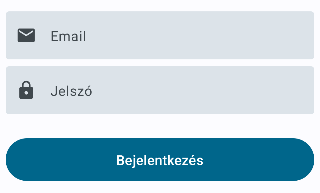
\includegraphics[width=0.5\linewidth]{images/login.png}
    \caption{Az elkészült Login panel.}
    \label{fig:finishedlogin}
\end{figure}

\section{OnlineCatchLog}

Ebben a szekcióban is a Model részletezésével kezdeném. Itt részletezni fogom a háttérfolyamatokat, amik lehetővé teszik az adatbázisom működését.
\subsection{Model}
\begin{itemize}
    \item \texttt{CatchLogDao}: A \textbf{@Dao} annotációval ellátott CatchLogDao egy Data Acces Object\cite{dao}, amely az adatbázisom műveleteit kezeli. Itt látjuk a metódusokat, amelyen keresztül kommunikálunk a Room adatbázissal.
    
\newpage
    
    \begin{java}[ caption = {CatchLogDao.kt részlet.}]
    @Dao
    interface CatchLogDao{
    
    }
    \end{java}
    \begin{itemize}
        \item \texttt{@Upsert}: Ez a metódus felelős azért, hogy egy új fogást rögzítsünk az adatbázisban. Másodlagosan ellenőrzi a meglévő rekordokat is.
\begin{java}
@Upsert
fun upsertCatchLog(catchLog: CatchLog)
\end{java}
        \item \texttt{@Query}: Az alábbi lekérdezéssel elérjük az összes eddig felvitt fogást az adatbázisban. Fontos, hogy ez a lekérdezés időrendi sorrendben valósul meg, azaz mindig a legfrissebb fogás lesz legfelül.
\begin{java}
@Query("SELECT * FROM catchlog ORDER BY catchTime ASC")
fun getLogsOrderedByTime(): Flow<List<CatchLog>>
\end{java}
    \end{itemize}

    \item \texttt{CatchLogEvent}: Ez a zárt interfész tartalmazza az eseményeket, amelyet az alkalmazás különböző részei felhasználhatnak az események kezelésére.
    Minden esemény külön adat osztályként, vagy objektumként van. Ezekkel tudunk az eseményekre reagálni.
    \begin{itemize}
        \item A \texttt{SaveCatchLog} esemény akkor hasznos, amikor frissen el szeretnénk menteni egy új kitöltött fogást.
        \item A \texttt{setLakeName, setLakeCode, setFishName, set FishWeight} pedig az adatmezőket frissítik.
        \item A \texttt{ShowDialog} illetve \texttt{HideDialog} a fogás felvitelét elindító folyamat részei. Amikor a képernyőn rá kattintunk az új fogás felvitelére ezen eseményekkel dolgozunk.
        \item A \texttt{SortLogs} eseménnyel pedig beállíthatjuk az adatbázis lekérdezésének típusát, sorrendjét.
        
\begin{java}[caption = { A CatchLogEvent eseményei. }]
sealed interface CatchLogEvent {
object SaveCatchLog
data class setLakeName(val lakeName: String)
data class setLakeCode(val lakeCode: Int)
data class setFishName(val fishName: String)
data class setFishWeight(val fishWeight: Int)
object ShowDialog
object HideDialog
data class SortLogs(val sortType: SortType)
}
\end{java}
    \end{itemize}
    \item \texttt{CatchLogDataBase}: Ezen a ponton viztosítjuk a Room adatbázis konfigurcióját.
    Először a \textbf{@Database} annotációval létrehozzuk az adatbázist. Ennek a feladata, hogy kezelje a CatchLog entitásokat, azaz a felvinni kívánt fogásokat. Ez az entitás magában foglalja a korábban említett adatokat, azaz a tó nevét, víztérkódját, hal nevét, súlyát, és a fogás időpontját. Ebben az osztályban továbbá megtalálható egy metódus, az \texttt{abstract val dao: CatchLogDao}. Ez biztosítja a hozzáférést a korábban említett \texttt{CatchLogDao} interfészhez, amellyel az alkalmazás a műveleteket fogja végrehajtani az adatbázison.

\begin{java}[caption = {CatchLogDataBase osztálya.}]
    @Database(
    entities = [CatchLog::class],
    version = 1
)
abstract class CatchLogDataBase: RoomDatabase() {
    abstract val dao: CatchLogDao
}
\end{java}
    \item \texttt{DataBaseModule}: Ez egy Dagger Hilt modul, amely biztosítja az adatbázist az egész alkalmazás számára. Itt részletezni szeretném a különböző komponenseket:
    \begin{itemize}
        \item \texttt{@Module} és \texttt{@InstallIn(SingletonComponent::class)} annotációk biztosítják azt, hogy a \texttt{DatabaseModule} globális függőségekkel segítse az alkalmazás többi elemét, és hogy hozzáférhező legyen az alkalmazás futása alatt.
        
\begin{java}[caption = {DataBaseModul-ban szereplő annotációk.}]
@Module
@InstallIn(SingletonComponent::class)
\end{java}

        \item \texttt{@Provides}: Ez a függőség segít létrehozni az adatbázist, amelyet később az alkalmazás az futása alatt használhat. Itt sajnos használnom kellett a \texttt{allowMainThreadQueries} metódust, ugyanis másképpen hibát produkált az alkalmazás. Ezt a későbbiekben fontos lenne kiküszöbölni, ugyanis az adatbázis így a fő processzor szálakon fut, ami a teljesítményünket negatív irányba eltolja. Ideális esetben ez a folyamat a háttérszálakon futna.
\begin{java}[caption = {provideCatchLogDataBase függőség.}]
@Provides
fun provideCatchLogDatabase(
@ApplicationContext context: Context):
CatchLogDataBase {
    return Room.databaseBuilder(
        context,
        CatchLogDataBase::class.java,
        "catch_log_database"
    ).allowMainThreadQueries().build()
}
\end{java}
        \item A \texttt{provieCatchLogDao} pedig elérhetővé teszi az alkalmazás többi részének az \texttt{CatchLogDao}-hoz való szükséges hozzáféréseket.
\begin{java}
@Provides
    fun provideCatchLogDao(
    database: CatchLogDataBase): CatchLogDao {
        return database.dao
    }
\end{java}
    \end{itemize}
    \item Végezetül pedig van egy egyszerű enum típusunk, a \texttt{SortType}. Ebben az Enum-ban deklarálhatunk új rendezési típusokat, ez jelen esetben csak az idő alapú Sort, azonban ez később könnyen bővíthető köszönhetően a felépítésnek.
\end{itemize}

\subsection{CatchLogViewModel}

Itt a programkód elején 2 fontos annotáció található. Az egyik a \texttt{@OptIn}, amellyel lehtővé tesszük az alkalmazás számára, hogy kísérleti fázisban lévő funkciókat használjunk. Ez ebben az esetben a \texttt{flatMapLatest}, és a \texttt{stateIn}. Ezek a funkciók az adat áramlásra, és az állapotkezelésre vonatkoznak.

A másik a \texttt{@HiltViewModel és @Inject}. Ezekről szó esett már korábban is, itt azonban más függőségeket injektálunk. Ezen a ponton a \texttt{Dao}-ot, ami egy adathozzáférési objetum a \texttt{CatchLogDao}-ban. Ezzel a művelettel közvetlen hozzá tud férni az adatbázis az előbbi programkódban leírt műveletekhez.

\begin{java}[caption = {Annotációk szemléletése.}]
@OptIn(ExperimentalCoroutinesApi::class)
@HiltViewModel    
\end{java}

Hasonlóan a korábbi ViewModel-ekhez itt is van egy \texttt{onAccountClick} metódus, amely egy másik kijelzőre hivatott átirányítani minket az \texttt{openAndPopUp} segítségével.

Ezután a ViewModel-ben kettő állapotáramlást kell létrehoznunk, a \texttt{\textunderscore sortType és \textunderscore cathLogs}-ot.
Ezekkel fogjuk kezelni a fogások listáját, valamint a korábban létrehozott rendezési sorrendet.
\begin{itemize}
    \item \texttt{\textunderscore sortType}: Ez egy \textbf{MutableStateFlow}, amely az aktuális rendezési típust tárolja. Ez estünkben a TIME, azaz idő szerinti sorolás.
    \item \texttt{\textunderscore catchLogs}: Ez pedig egy \textbf{StateFlow}, ami a \textbf{\textunderscore sortType} flow változásaira reagál. Ha hozzáadunk többféle rendezési típust az alkalmazásunkhoz, akkor a \textbf{flatMapLatest} segítségével egy újabb lekérdezést valósíthatunk meg.

\newpage

\begin{java}[caption = {A különböző Flow típusok szemléltetése.}]
private val _sortType = MutableStateFlow(SortType.TIME)
private val _catchLogs = _sortType
    .flatMapLatest { sortType ->
        when(sortType) {
            SortType.TIME -> dao.getLogsOrderedByTime()
        }
    }
    .stateIn(viewModelScope,
    SharingStarted.WhileSubscribed(), emptyList())
    
\end{java}
\end{itemize}

 A state kombinálja a \textunderscore state, \textunderscore sortType, \textunderscore catchLogs flow-kat.
 \begin{itemize}
     \item \texttt{combine}: Ez a flow figyeli mindhárom áramlás aktuális állapotát. Ha bármelyikük megváltozik a state frissül.
     \item \texttt{stateIn}: Ez a metódus biztosítja azt, hogy a state állapotáramlása a ViewModel használatához legyen kötve, ezáltal mindig elérhető marad. Tehát amíg használjuk ezt a kijelzőt, addig fog működni. Miután nem használja az alkalmazás 5 másodpercig, a stateIn megszűnik.

\begin{java} [caption = {A combine szemléltetése.}]
private val _state = MutableStateFlow(CatchLogState())
val state = combine(_state, _sortType, _catchLogs)
    { state, sortType, catchLogs ->
    state.copy(
        catchLogs = catchLogs,
        sortType = sortType
    )
}.stateIn(viewModelScope,
SharingStarted.WhileSubscribed(5000),
CatchLogState())

\end{java}
\end{itemize}

Ezen a ponton jutunk el, az \textbf{onEvent()}-re. Ez a metódus kezelei a fogási napló eseményeket, amelyek különböző felhasználói tevékenységeket jelznek. Itt egy \texttt{when} ággal dolgozunk, és minden különböző eseménytípusnál különböző műveletet hajtunk végre.
\begin{itemize}
    \item \texttt{Hide-ShowCatalog}: Ez a korábban említett függvény végzi a dialógus előhozatalát, és elrakását. Ezt abban az esetben hívjuk meg ha a felhasználó új adatot akar felvinni a táblázatba, azaz naplózni szeretné a fogását. Abban az esetben pedig elrejtjük, ha feltöltött egy fogást, vagy félbe hagyja a fogás feltöltését.
    \item A \texttt{set} előváltozóval ellátott események felelősek azért, hogy az állapotot frissítsék az új mező értékével. Azaz amit leírunk, azt lássuk is.
\begin{java}
is CatchLogEvent.setFishWeight -> {
    _state.update { 
        it.copy(fishWeight = event.fishWeight) }
}
\end{java}

    \item \texttt{SaveCatchLog}: Ez az az esemény, amely a formában lévő adatokat sikeresen kitöltés esetés lementi. Ebből adódóan először ellenőrzi, hogy a \texttt{lakeName, fishName} helyesek-e, illetve hogy meg legyenek adva.
\begin{java}
CatchLogEvent.SaveCatchLog -> {
            val lakeName = state.value.lakeName
            val lakeCode = state.value.lakeCode
            val fishName = state.value.fishName
            val fishWeight = state.value.fishWeight

            if(lakeName.isBlank() || fishName.isBlank()) {
                return
            }
        }
\end{java}

    Ha az előfeltételek teljesültek, azaz helyesek az adatok és nem hagytunk üresen mezőt, akkor létrehoz egy \textbf{CatchLog} objektumot, és aszinkron módba lementi a korábban létrehozott \texttt{dao.upsertCatchLog} segítségével.
\begin{java}
viewModelScope.launch {
        dao.upsertCatchLog(catchLog)
        }
\end{java}
    Ezek után kiüríti az előbb használt mezőket, majd eltünteti a dialógust.
\end{itemize}

\subsection{OnlineCatchLogView}

Ezen a ponton elérkeztünk a CatchLog szakasz View komponenséhez. A korábban tárgyalt metódusokra csak említés szinjtén szeretnék kitérni, az újakat pedig részletezem.

\begin{itemize}
    \item \textbf{Scaffold:} Ez a Column-tól eltérően egy általános elrendezési eljárás. Itt csak egy alapvető struktúrát biztosítunk az alkalmazásnak, amin keresztül meg tud jeleníteni. Ezen belül találunk egy \texttt{topBar}-t, ami a kijelző felső részén egy sávot hoz létre, amit szabadon testreszabhatunk. A következő deklaráció a 
    \newline
    \texttt{floatingActionButton}, ami a kijelző alján egy "lebegő" gombot hoz létre, amivel interaktálhatunk.
\begin{figure} [h]
\centering

\includegraphics[width=0.5\linewidth]{images/floatingactionbutton.png}
\caption{A "lebegő" gomb.}
\label{fig:floatingactionbutton}
\end{figure}
\newpage

\begin{java} [caption = { A topBar szemléltetése.}]
topBar = {
    TopAppBar(
    title = { Text(stringResource(R.string.app_name)) },
    actions = {
        IconButton(onClick = {
            viewModel.onAccountClick(openAndPopUp) }) {
            Icon(Icons.Filled.AccountCircle,
                "Account")
            }
        }
    )
} 
\end{java}
Ezen belül láthatjuk, hogyan is épül fel a \texttt{topBar}.
Tudunk neki nevet adni a \textbf{title} változó segítségével, ami a korábban említett \textbf{Stringek} közül kerül kiválasztásra, amit már előre megírtunk.
Egyel lejebb az \textbf{actions}-nél itt is észrevehetjük, hogy az \texttt{openAndPopUp} metódust hívjuk meg. Ez azért van, mert egy gomb található ebben a szekcióban, amivel átirányítjuk a felhasználót az \textbf{Account} oldalra. végezetül pedig a kattintható gombnak adunk egy ikont.

\begin{java} [caption = {A lebegő gomb programbeli megvalósítása.}]
 floatingActionButton = {
    FloatingActionButton(onClick = {
         onEvent(CatchLogEvent.ShowDialog)
    }) {
        Icon(
            imageVector = Icons.Default.Add,
            contentDescription = "Fogas"
        )
    }
}
\end{java}

A \texttt{floatingActionButton}-nál hasonló a helyzet. Itt azonban nem irányítjuk át a felhasználót egy másik oldalra, hanem felkinálunk neki egy dialógust, ugyanis ezzel a gombbal lehet megnyitni az adatfeltöltést. Itt beállítjuk a gomb ikonját, ami a mi esetünkben egy \textbf{+} jel lesz. Ezzel is törekszünk alkalmazásunk intuivitásának fenntartására.

\item \textbf{LazyColumn}: Ez a sima Column-tól eltérően csak akkor tölti be az elemeket, ha megjelennek a képernyőn. Ez abból a szempontból fontos, hogy valószínű a felhasználónak nem 2-3 feltöltött fogása lesz, hanem valószínű több száz. Így erőforrásokat spórolhatunk, mivel nem töltjük be az összes fogást egyszerre.

Láthatjuk, hogy a betöltés csak egyszer szerepel. Ez annyiszor fut le, ahány fogást be kell töltenie az alkalmazásnak. A fontosabb információk nagyobb betűmérettel rendelkeznek, még a kevésbé fontosak, (például: víztérkód) kevésbé látszanak. Ezzel azt próbáljuk elősegíteni, hogy jobban átláthatóbb legyen a kezelői felület.
\end{itemize}

\newpage

\subsection{AddLogDialog}

Az AddLogDialog majdnem egy külön komponenst képez. Ide leszünk át irányítva a lebegő gomb megnyomása után. Közvetlenül nem egy új ablak, hanem egy dialógus. Nézzük meg részletesebben.

 \texttt{AlertDialog}: Ez biztosítja a felugró ablakot. Három fő része van. Az első az onDissmissRequest, ahol meghatározzuk, hogy mi történjen, amikor a User megkíséreli bezárni a dialógust. Ezután a \texttt{CatchLogEvent.HideDialog} eseménnyel tájékoztatjuk a viewModel-t a dialógus bezárásáról. A második elem a \texttt{title}, amivel értelemszerűen címet adhatunk a dialógusunknak. Ez nálam a "Fogás hozzáadása". A harmadik pedig a \textbf{text}, amellyel Column elrendezésben, azaz egymás alatt megnevezhetjük a beviteli mezők feladatát.

\begin{java}[caption = {Az AlertDialog felépítési váza.}]
AlertDialog(
    modifier = modifier,
    onDismissRequest = {
        onEvent(CatchLogEvent.HideDialog)
    },
    title = { },
    text = { },
    buttons = { }
)
\end{java}

\texttt{Textfield}: Hasonlóan a bejelentkezési kijelzőhöz, itt is beviteli módként ezeket használom.
A \texttt{value} a beviteli mező tartalma, ez a \texttt{state.lakeName} alapján frissül.
Az \texttt{onValueChange} lényege, hogy ha a felhasználó bevisz egy adatot, akkor a \texttt{CatchLogEvent.setLakeName} hívjuk meg, ami frissíti a bevitt adattal az állapotot.
A \texttt{placeholder} pedig hasonlóan a korábbi példával iránymutatást ad a \texttt{textField} használatával kapcsolatban.

\begin{java}[caption = {A lakeName beviteli mező.}]
 TextField(
            value = state.lakeName,
            onValueChange = {
                onEvent(CatchLogEvent.setLakeName(it))
            },
            placeholder = {
                Text(text = "To megnevezese")
            }
        )    
\end{java}

Ettől egy részen eltér a víztérkód, és a hal súlya mező. Ugyanis ezeknek a típusa Int, ahol nem lenne ésszerű felkínálni a teljes billentyűzetet a felhasználónak. Ezért a könnyebb bevitelt hivatott elősegíteni a \texttt{KeyboardType.Number}. Ennek a lényege az, hogy a User csak egy numerikus billentyűzetet fog kapni, amivel kifejezetten csak számokat tud bevinni a mezőbe.

\newpage

\begin{java}[caption = {A víztérkód programrészlet szemléltetése.}]
TextField(
    value = state.lakeCode.toString(),
    onValueChange = {
        val lakeCodeInt = it.toIntOrNull()
        if (lakeCodeInt != null) {
            onEvent(CatchLogEvent.setLakeCode(lakeCodeInt))
        } else { }
    },
    placeholder = {
        Text(text = "Vizterkod")
    },
    keyboardOptions = KeyboardOptions(
        keyboardType = KeyboardType.Number)
)    
\end{java}

\section{Account}
Itt elérkeztünk ennek a fejezet utolsó szekciójához, a fiókhoz. Itt kettő dolgot kellett megvalósítanom. Először is, fontos hogy a felhasználó itt ki tudjon jelentkezni az alkalmazásból. 
Másodszor pedig fel kellett kínálni egy lehetőséget arra, hogy vissza tudjunk menni a fogási napló részre.

Itt nem részeletném a Model részét a fióknak, ugyanis az a része megegyezik a bejelentkező szekcióval.

\subsection{AccountViewModel}

Az \texttt{initialize} felelős az alkalmazás ujraindításáért miután kijelentkeztetjük a felhasználót.
Ezen belül található a \texttt{restartApp} függvény, amely vissza küldi a felhasználót a Splash kijelzóre.
Ebben a blokkban a \texttt{launchCatching}-en belül az
\newline
\texttt{accountService.currentUser} folyamatot figyeli. Amint kijelentkeztetjük a felhasználót ez \texttt{null} állapotú lesz. Ezután aktiválódik a \texttt{restartApp}.

\begin{java}
fun initialize(restartApp: (String) -> Unit) {
    launchCatching {
        accountService.currentUser.collect { user ->
            if (user == null) restartApp(SPLASH_SCREEN)
        }
    }
}

\end{java}

\newpage

Ezután láthatjuk ezen szekció kettő fő függvényét.
Az első az \texttt{onSignOutClick}. Ez jelentkezteti ki a felhasználót az \texttt{accountService.signOut()} meghívásával.

\begin{java}
fun onSignOutClick() {
    launchCatching {
        accountService.signOut()
    }
}
\end{java}

A második az \texttt{onCatchLogClick}, ami vissza irányítja a felhasználót a fogási napló oldalára, és törli a stack-ből a jelenlegi kijelzőt.

\begin{java}
fun onCatchLogClick(openAndPopUp: (String, String) -> Unit){
    launchCatching {
        openAndPopUp(CATCHLOG_SCREEN, ACCOUNT_SCREEN)
    }
}    
\end{java}

\subsection{AccountView}

Itt a programkód eleje a \texttt{LaunchedEffect}-el kezdődik. Ezen a blokkon belül hívjuk meg a korábban létrehozott\texttt{initialize}-t. Ez biztosítja, hogy ha nincs bejelentkezett felhasználó, akkor vissza kerülönk a bejelentkezés oldalra.

\begin{java}
LaunchedEffect(Unit) { viewModel.initialize(restartApp) }
\end{java}

Továbbá létrehozunk a \texttt{showExitAppDialog}-ot, ami \textbf{mutableStateOf(false)} kezdeti értékkel létrehoz egy állapotot. Ez azt fogja jelezni az alkalmazásnak, hogy a kijelentkezési dialógus meg jelenjen-e.

\begin{java}
var showExitAppDialog by remember { mutableStateOf(false) }
\end{java}

A \texttt{TopAppBar} változó itt hasonlóan az előző szekcióban említettekkel az
\newline
\texttt{openAndPopUp}
metódussal vissza vezeti a felhasználót az előző oldalra.

\begin{java}
TopAppBar(
    title = { Text(stringResource(R.string.app_name)) },
    actions = {
        IconButton(onClick = { 
            viewModel.onCatchLogClick(openAndPopUp) }) {
            Icon(Icons.Filled.ArrowBack, "Catch log")
        }
    }
)
\end{java}

A képernyő közepén egy szimpla gomb található, aminek az a feladata, hogy kijelentkeztesse a felhasználót. Amint erre rákattintunk a \texttt{showExitAppDialog} értéke igaz lesz, így megjelenik a dialógusunk.
\newpage
A dialógus megjelenítésért az \texttt{AlertDialog} függvény gondoskodik. Itt a felhasználónak kettő opciót ajánlunk fel. Az első opcióban megszakíthatja a kijelentkezés folyamatát, így bent marad az alkalmazásban, és nem kell újra bejelentkeznie. A második opció a kijelentkezés megerősítése. Ebben az esetben a felhasználó vissza lesz irányítva a bejelentkezés oldalra, ahol ismét meg kell adnia az adatait, vagy át adhatja a telefonját és bejelentkezhet a horgásztársa.

\begin{java}
AlertDialog(
    title={Text(stringResource(R.string.sign_out_title))},
    text={Text(stringResource(R.string.sign_out_description))},
    dismissButton = {
        Button(onClick = { showExitAppDialog = false }) {
            Text(text = stringResource(R.string.cancel))
        }
    },
    confirmButton = {
        Button(onClick = {
            viewModel.onSignOutClick()
            showExitAppDialog = false
        }) {
            Text(text = stringResource(R.string.sign_out))
        }
    },
    onDismissRequest = { showExitAppDialog = false }
)
\end{java}